\documentclass[12pt]{article}

%%%%%%%%%%%%%%%%%%%%%%%%%%%%%%%%%%%%%%%%%%%%%%%%%%%%%%%%%%%%%%%%%%%%%%%%%%%%%%%%
%                           Package preset for homework
%%%%%%%%%%%%%%%%%%%%%%%%%%%%%%%%%%%%%%%%%%%%%%%%%%%%%%%%%%%%%%%%%%%%%%%%%%%%%%%%
% Miscellaneous
\usepackage[margin=1in]{geometry}
\usepackage[utf8]{inputenc}
\usepackage{indentfirst}
\usepackage{blindtext}
\usepackage{graphicx}
\usepackage{xr-hyper}
\usepackage{hyperref}
\usepackage{enumitem}
\usepackage{color}
\usepackage{float}
% Math
\usepackage{latexsym}
\usepackage{amsfonts}
\usepackage{amssymb}
\usepackage{amsmath}
\usepackage{commath}
\usepackage{amsthm}
\usepackage{bbold}
\usepackage{bm}
% Physics
\usepackage{physics}
\usepackage{siunitx}
% Code typesetting
\usepackage{listings}
% Citation
\usepackage[authoryear]{natbib}
\usepackage{appendix}
\usepackage[capitalize]{cleveref}
% Title & name
\title{Homework}
\author{Tien Vo}
\date{\today}


%%%%%%%%%%%%%%%%%%%%%%%%%%%%%%%%%%%%%%%%%%%%%%%%%%%%%%%%%%%%%%%%%%%%%%%%%%%%%%%%
%                   User-defined commands and environments
%%%%%%%%%%%%%%%%%%%%%%%%%%%%%%%%%%%%%%%%%%%%%%%%%%%%%%%%%%%%%%%%%%%%%%%%%%%%%%%%
%%% Misc
\sisetup{load-configurations=abbreviations}
\newcommand{\due}[1]{\date{Due: #1}}
\newcommand{\hint}{\textit{Hint}}
\let\oldt\t
\renewcommand{\t}[1]{\text{#1}}

%%% Bold sets & abbrv
\newcommand{\N}{\mathbb{N}}
\newcommand{\Z}{\mathbb{Z}}
\newcommand{\R}{\mathbb{R}}
\newcommand{\Q}{\mathbb{Q}}
\let\oldP\P
\renewcommand{\P}{\mathbb{P}}
\newcommand{\LL}{\mathcal{L}}
\newcommand{\FF}{\mathcal{F}}
\newcommand{\HH}{\mathcal{H}}
\newcommand{\NN}{\mathcal{N}}
\newcommand{\ZZ}{\mathcal{Z}}
\newcommand{\RN}[1]{\textup{\uppercase\expandafter{\romannumeral#1}}}
\newcommand{\ua}{\uparrow}
\newcommand{\da}{\downarrow}

%%% Unit vectors
\newcommand{\xhat}{\vb{\hat{x}}}
\newcommand{\yhat}{\vb{\hat{y}}}
\newcommand{\zhat}{\vb{\hat{z}}}
\newcommand{\nhat}{\vb{\hat{n}}}
\newcommand{\rhat}{\vb{\hat{r}}}
\newcommand{\phihat}{\bm{\hat{\phi}}}
\newcommand{\thetahat}{\bm{\hat{\theta}}}

%%% Other math stuff
\providecommand{\units}[1]{\,\ensuremath{\mathrm{#1}}\xspace}
% Set new style for problem
\newtheoremstyle{problemstyle}  % <name>
        {10pt}                   % <space above>
        {10pt}                   % <space below>
        {\normalfont}           % <body font>
        {}                      % <indent amount}
        {\bfseries\itshape}     % <theorem head font>
        {\normalfont\bfseries:} % <punctuation after theorem head>
        {.5em}                  % <space after theorem head>
        {}                      % <theorem head spec (can be left empty, 
                                % meaning `normal')>

% Set problem environment
\theoremstyle{problemstyle}
\newtheorem{problemenv}{Problem}[section]
\newenvironment{problem}[1]{%
  \renewcommand\theproblemenv{#1}%
  \problemenv
}{\endproblemenv}
% Set lemma environment
\newenvironment{lemma}[2][Lemma]{\begin{trivlist}
\item[\hskip \labelsep {\bfseries #1}\hskip \labelsep {\bfseries #2.}]}{\end{trivlist}}
% Set solution environment
\newenvironment{solution}{
    \begin{proof}[Solution]$ $\par\nobreak\ignorespaces
}{\end{proof}}
\numberwithin{equation}{problemenv}

%%% Page format
\setlength{\parindent}{0.5cm}
\setlength{\oddsidemargin}{0in}
\setlength{\textwidth}{6.5in}
\setlength{\textheight}{8.8in}
\setlength{\topmargin}{0in}
\setlength{\headheight}{18pt}

%%% Code environments
\definecolor{dkgreen}{rgb}{0,0.6,0}
\definecolor{gray}{rgb}{0.5,0.5,0.5}
\definecolor{mauve}{rgb}{0.58,0,0.82}
\lstset{frame=tb,
  language=Python,
  aboveskip=3mm,
  belowskip=3mm,
  showstringspaces=false,
  columns=flexible,
  basicstyle={\small\ttfamily},
  numbers=none,
  numberstyle=\tiny\color{gray},
  keywordstyle=\color{blue},
  commentstyle=\color{dkgreen},
  stringstyle=\color{mauve},
  breaklines=true,
  breakatwhitespace=true,
  tabsize=4
}
\lstset{
  language=Mathematica,
  numbers=left,
  numberstyle=\tiny\color{gray},
  numbersep=5pt,
  breaklines=true,
  captionpos={t},
  frame={lines},
  rulecolor=\color{black},
  framerule=0.5pt,
  columns=flexible,
  tabsize=2
}


\title{Homework 5: Phys 7320 (Spring 2022)}
\due{February 16, 2022}

\begin{document}
\maketitle
%%%%%%%%%%%%%%%%%%%%%%%%%%%%%%%%%%%%%%%%%%%%%%%%%%%%%%%%%%%%%%%%%%%%%%%%%%%%%%%
\begin{problem}{5.1}[Fresnel Diffraction]
A perfectly conducting flat screen occupies half of the $xy$ plane (i.e.,
$x<0$). A plane wave of intensity $I_0$ and wave number $k$ is incident along
the $z$ axis from the region $z<0$. Discuss the values of the diffracted fields
in the plane parallel to the $xy$ plane defined by $z=Z>0$. Let the coordinates
of the observation point be $(X,0,Z)$.

(a) Show that, for the usual scalar Kirchhoff approximation and in the limit
$Z\gg X$ and $\sqrt{kZ}\gg1$, the diffracted field is
\begin{equation}
    \psi(X,0,Z,t)\approx
    I_0^{1/2}e^{ikZ-i\omega t}\qty(\frac{1+i}{2i})
    \sqrt{\frac2\pi}\int_{-\xi}^\infty e^{it^2}dt
\end{equation}
where $\xi=(k/2Z)^{1/2}X$.

(b) Show that the intensity can be written
\begin{equation}
    I=\abs{\psi}^2=\frac{I_0}{2}\qty[\qty(C(\xi)+\frac12)^2+\qty(S(\xi)+\frac12)^2] 
\end{equation}
where $C(\xi)$ and $S(\xi)$ are the so-called Fresnel integrals. Determine the
asymptotic behavior of $I$ for $\xi$ large and positive (illuminated region) and
$\xi$ large and negative (shadow region). What is the value of $I$ at $X=0$?
Make a sketch of $I$ as a function of $X$ for fixed $Z$.

\textit{Hint}: Use the Dirichlet (``generalized'') version of the Kirchhoff
integral as in class or Jackson (10.85), with the subleading $+i/(kR)$
neglected, and expand
\begin{equation}
    R=\qty[(x-x')+y'^2+z^2]^{1/2}\approx
    z\qty[1+\frac{(x-x')^2+y'^2}{2z^2}+\hdots].
\end{equation}
There are several definitions of Fresnel integrals with slightly different
conventions. The Abramowitz and Stegun definition is
\begin{equation}
    C(u)=\sqrt{\frac2\pi}\int_0^udt\cos(t^2),
    \qquad
    S(u)=\sqrt{\frac2\pi}\int_0^u dt\sin(t^2).
\end{equation}
Note that in the result Jackson quotes for part (a), $t$ is used for two
completely different things -- in $e^{-i\omega t}$ it is the time, while in
$e^{it^2}dt$ it is an integration variable related to $x$ and $x'$. This is
obviously terrible; the time dependence is just the usual harmonic dependence
and plays no further role.
\begin{solution}
(a) First, we expand the distance $R=\sqrt{(X-x')^2+y'^2+Z^2}$ as hinted.
\begin{equation}
    R=Z\sqrt{1+\frac{(X-x')^2+y'^2}{Z^2}}
    \approx Z\qty[1+\frac{(X-x')^2+y'^2}{2Z^2}].
\end{equation}
Then, as $Z$ is large, $R\sim Z$ and $kR\ll 1$. The generalized Kirchhoff
integral (10.85, Jackson) can be written as
\begin{align}\label{p1:psi}
    \psi
    &=\frac{kZ}{2\pi i}\int_{S_1}\frac{e^{ikR}}{R^2}\psi(\vb{x}')dx'dy',
\end{align}
where $S_1=\qty{(x,y,0)|x,y\in\R\wedge x\geq0}$. On $S_1$,
$\psi$ assumes the form without the conducting screen
$\psi=\psi_0e^{-i\omega t}$ where $\psi_0^2=I_0$. It follows that
\begin{align}
    \psi
    &\approx \sqrt{I_0}\frac{k}{2\pi iZ}e^{i(kZ-\omega t)}
    \int_{-\infty}^\infty dy'e^{(1/2)i(k/Z)y'^2}
    \int_0^\infty dx' e^{ik(X-x')^2/2Z}\notag\\
    &=\sqrt{I_0}\frac1{2\pi i}\frac{k}{Z}e^{i(kZ-\omega t)}
        \sqrt{\frac{2\pi}{-ik/Z}}\int_{X\sqrt{k/2Z}}^{-\infty}\qty(-\sqrt{\frac{2Z}{k}})du
        e^{iu^2}\tag{$u^2=k(X-x')^2/2Z$}\\
    &=\sqrt{I_0}\frac{1}{\sqrt\pi}\frac1{i\sqrt{-i}}e^{i(kZ-\omega t)}
    \int_{-\xi}^\infty due^{iu^2}\tag{$\xi=X\sqrt{k/2Z}$}\notag\\
    &=\sqrt{I_0}e^{i(kZ-\omega t)}\frac{1+i}{2i}\sqrt{\frac2\pi}
    \int_{-\xi}^\infty du e^{iu^2}
\end{align}
where $1/i\sqrt{-i}=(1/\sqrt2)(1-i)$. This is the desired result.

(b) First, note that
\begin{equation}\label{p1b:lim}
    \lim_{u\to\infty}C(u)=\lim_{u\to\infty}S(u)=\frac12 ,
\end{equation}
from the Abramowitz \& Stegun definition. Then, we can rewrite our result for
$\psi$ in (a) as
\begin{align}
    \psi
    &=I_0^{1/2}e^{i(kZ-\omega t)}\frac{1+i}{2i}\sqrt{\frac2\pi}
    \qty(\int_0^\xi due^{iu^2}+\int_0^\infty du e^{iu^2})\notag\\
    &=I_0^{1/2}e^{i(kZ-\omega t)}\frac{1+i}{2i}
    \qty[C(\xi)+iS(\xi)+C_\infty+iS_\infty]\notag\\
    &=I_0^{1/2}e^{i(kZ-\omega
    t)}\frac12\qty(1-i)\qty[\qty(C(\xi)+\frac12)+i\qty(S(\xi)+\frac12)].
\end{align}
Then, it is trivial to calculate
\begin{align}
    I=\abs{\psi}^2
     =\frac{I_0}{2}\qty[\qty(C(\xi)+\frac12)^2+\qty(S(\xi)+\frac12)^2].
\end{align}
From \eqref{p1b:lim}, $\lim_{\xi\to\infty}I=I_0$. However, at the opposite
limit,
\begin{equation}
    \lim_{u\to-\infty}C(u)=\lim_{u\to-\infty}S(u)=-\frac12 .
\end{equation}
Thus, $\lim_{\xi\to-\infty}I=0$. At $X=\xi=0$, it is clear from the bounds of
the Fresnel integrals that $C(0)=S(0)=0$. So $I(\xi=0)=I_0/4$. A plot of $I$ is
shown below where the limiting behavior and the value of $I$ at $\xi=0$ are
confirmed.
\begin{center}
    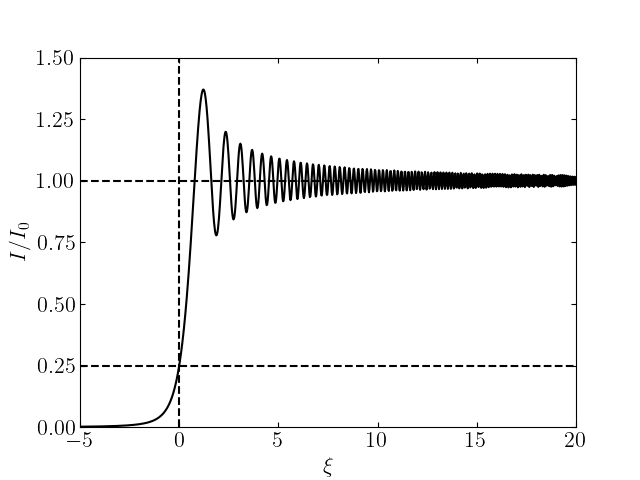
\includegraphics[width=0.8\textwidth]{p1b.png} 
\end{center}
\end{solution}
\end{problem}
\newpage
%%%%%%%%%%%%%%%%%%%%%%%%%%%%%%%%%%%%%%%%%%%%%%%%%%%%%%%%%%%%%%%%%%%%%%%%%%%%%%%    
%%%%%%%%%%%%%%%%%%%%%%%%%%%%%%%%%%%%%%%%%%%%%%%%%%%%%%%%%%%%%%%%%%%%%%%%%%%%%%%
\begin{problem}{5.2}[Diffraction through a circular hole]
A linearly polarized plane wave of amplitude $E_0$ and wave number $k$ is
incident on a circular opening of radius $a$ in an otherwise perfectly
conducting flat screen. The incident wave vector makes an angle $\alpha$ with
the normal to the screen. The polarization vector is perpendicular to the plane
of incidence.

(a) Calculate the diffracted fields and the power per unit solid angle
transmitted through the opening, using the vector Smythe-Kirchhoff formula
(10.101) with the assumption that the tangential electric field in the opening
is the unperturbed incident field.

(b) Compare your result in part (a) with the standard scalar Kirchhoff
approximation and with the result in Section 10.9 for the polarization vector in
the plane of incidence.

\textit{Hint}: In (a), work in the Fraunhofer limit. In class (also Jackson pp.
491--492), we discussed the same case except the initial polarization was in the
plane of incidence; now on this homework problem the initial polarization is
perpendicular to the plane of incidence, $\bm\epsilon_0=\yhat$. Go through the
steps and fill out details. For part (b), again use the Dirichet Kirchhoff
formula with the subleading $+i/(kR)$ dropped.
\begin{solution}
(a) First, the incident electric field can be written as
\begin{equation}
    \vb{E}_i=E_0\yhat e^{ik(\sin\alpha x+\cos\alpha z)}. 
\end{equation}
So, with a normal $\nhat=\zhat$, 
\begin{equation}
    \nhat\vdot\vb{E}(\vb{x}')=-E_0\xhat e^{ik\sin\alpha x'}
    =-E_0\xhat e^{ik\rho\sin\alpha\cos\beta},
\end{equation}
where $\vb{x}'\in S_1$ and $x'=\rho\cos\beta$. Now, plugging into (10.109,
Jackson), we get
\begin{align}
    \vb{E}(\vb{x})
    &=\frac{-ie^{ikr}}{2\pi r}E_0(\vb{k}\times\xhat)
    \int_{S_1}\rho d\rho d\beta e^{ik\rho\sin\alpha\cos\beta}
    e^{-ik\rho(\sin\theta\cos(\phi-\beta))}.
\end{align}
Performing a change of variable
$\xi=(\sin^2\theta+\sin^2\alpha-2\sin\theta\sin\alpha\cos\phi)^{1/2}$, we can
calculate
\begin{equation}
    \vb{E}(\vb{x})
    =-\frac{ie^{ikr}E_0}{2\pi r}\qty(\vb{k}\times\xhat)
    \int_0^a\rho d\rho 2\pi J_0(k\rho\xi)
    =-ie^{ikr}E_0\frac{a}{r}\qty(\vb{\hat{k}}\times\xhat)\frac{J_1(ka\xi)}{\xi},
\end{equation}
where $\vb{\hat{k}}\times\xhat=-\sin\theta\sin\phi\zhat+\cos\theta\zhat$. It
then follows that
\begin{equation}
    \abs{\vb{E}}^2=\qty(\frac{a}{r})^2E_0^2\qty(\cos^2\theta+\sin^2\theta\sin^2\phi)\abs{\frac{J_1(ka\xi)}{\xi}}^2,
\end{equation}
and from (9.21, Jackson), 
\begin{align}\label{p2a:dP}
    \frac{dP}{d\Omega}
    &=\frac{r^2}{2Z_0}\abs{\vb{E}}^2\notag\\
    &=\frac{P_i}{\pi\cos\alpha}(\cos^2\theta+\sin^2\theta\sin^2\phi)\abs{\frac{J_1(ka\xi)}{\xi}}^2\notag\\
    &=P_i\frac{(ka)^2}{4\pi\cos\alpha}(\cos^2\theta+\sin^2\theta\sin^2\phi)\abs{\frac{2J_1(ka\xi)}{ka\xi}}^2
\end{align}
where $P_i=(E_0^2/2Z_0)\pi a^2\cos\alpha$ is defined in (10.115).

(b) First, we note that at $\alpha=0$, $\xi=\sin\theta$ and \eqref{p2a:dP} 
reduces to
\begin{equation}\label{p2b:dP}
    \frac{dP}{d\Omega}
    =\frac{P_i}{\pi}\abs{\frac{J_1(ka\sin\theta)}{\tan\theta}}^2
    \approx\frac{P_i}{\pi}\abs{\frac{J_1(ka\sin\theta)}{\sin\theta}}^2.
\end{equation}
since $\theta$ is restricted to a very small forward angle ($\theta\ll 1$).
(10.114) would also reduce to the same form since the 
$\cos^2\phi\sin^2\theta$ term would vanish. Now, we derive the radiation 
pattern with scalar diffraction theory. Recall from \eqref{p1:psi},
\begin{equation}\label{p2:psi}
    E=\frac{kz}{2\pi i}\int_{S_1}\frac{e^{ikR}}{R^2}\psi(\vb{x}')\rho d\rho
    d\beta 
\end{equation}
where $S_1$ is the circular hole. $\psi$ on $S_1$ is
\begin{equation}
    \psi(\vb{x}')=E_0 e^{i(\vb{k}_0\vdot\vb{x}'-\omega t)}
    E_0e^{-i\omega t}e^{ik\sin\alpha x'}
    =E_0e^{-i\omega t}e^{ik\rho\sin\alpha\cos\beta},
\end{equation}
while $kR\approx kr-\vb{k}\vdot\vb{x}'=kr-k\rho\sin\theta\cos\qty(\phi-\beta)$.
Plugging back into \eqref{p2:psi}, we get
\begin{equation}
    E=\frac{kz}{2\pi i}E_0\frac{e^{i(kr-\omega t)}}{r^2}\int_0^a\rho
    d\rho\int_0^{2\pi}d\beta
    e^{ik\rho(\sin\alpha\cos\beta-\sin\theta\cos(\phi-\beta))}.
\end{equation}
We have solved this integration before. The result is
\begin{align}
    E
    &=\frac{kz}{i}E_0e^{i(kr-\omega t)}\frac{a^2}{r^2}\frac{J_1(ka\xi)}{ka\xi}
    \notag\\
    &=-ie^{i(kr-\omega t)}E_0\frac{a}{r}\cos\theta\frac{J_1(ka\xi)}{\xi}
\end{align}
Then, the radiation pattern is
\begin{equation}
    \frac{dP}{d\Omega}
    =\frac{r^2}{2Z_0}\abs{E}^2
    =\frac{a^2E_0^2}{2Z_0}\cos^2\theta\abs{\frac{J_1(ka\xi)}{\xi}}^2
    =\frac{P_i}{\pi\cos\alpha}\cos^2\theta\abs{\frac{J_1(ka\xi)}{\xi}}^2
\end{equation}
Once again, at $\alpha=0$ and $\theta\ll 1$, this result reduces to
\eqref{p2b:dP}. So all scalar and vector approximations reduce to the common
expression (10.120, Jackson), as expected. Regarding their similarities, we
observe that they all scale as $\abs{J_1/\xi}^2$.
\end{solution}
\end{problem}
\newpage
%%%%%%%%%%%%%%%%%%%%%%%%%%%%%%%%%%%%%%%%%%%%%%%%%%%%%%%%%%%%%%%%%%%%%%%%%%%%%%%
\end{document}
